\section*{Problema 1}
Tomando la ecuación de movimiento para un objeto en caida libre con resistencia cuadrática
	$$ \dv{p}{t} = mg - kv^2, $$
para un coeficiente de resistencia $k = 10^{-4}$ y una masa de $10g$, se utilizó el método de runge kutta para resolver la ecuación. Se tomó un paso de $h = 0.1$ y se comparó con la solución analítica para un movimiento sin resistencia del aire.

\begin{figure}[H]
	\centering
	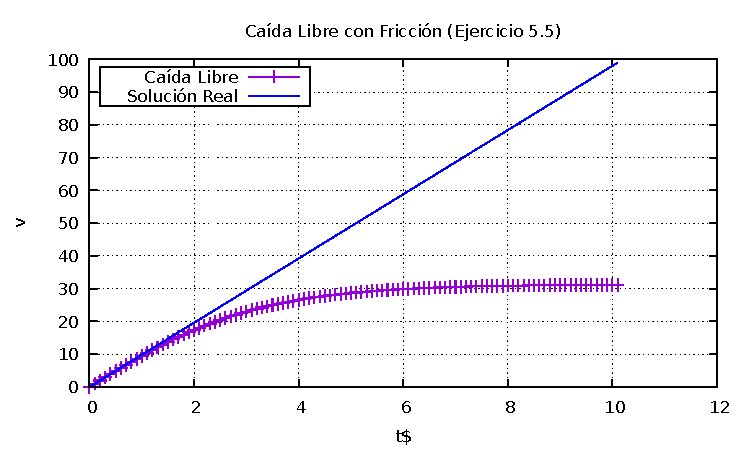
\includegraphics[scale=1]{../img/ej5-5.pdf}
	\caption{Solución utilizando el método de Runge Kutta comparada con la solución real ignorando la resistencia del aire.}
	\label{ej5-5}
\end{figure}

En la figura \ref{ej5-5} es clara la implicación de la resistencia del aire, puesto que se tiene una asíntota en aproximadamente $32m/s$, la cual es conocida como la velocidad terminal. Cosa que para el movimiento sin resistencia del aire, no se tiene.

\begin{lstlisting}
// Librerias
#include <iostream>
#include <fstream>
#include <cmath>
#include <iomanip>

using namespace std;

void RK4(const double *y,
        const int n_ec,
        const double t,
        const double h,
        double *y_new,
          void (*derivada)(const double *, const double, double *));
void salidaSolucion(const double t, const double *y, const int N);
void oneD_ProjectileMotion(const double *y, const double t, double *dydt);


int main(){
  // Datos iniciales
  const double t0 = 0.0;
  const double y0 = 0.0;
  const double h = 0.1;
  const int N = 10/h; // numero de iteraciones
  const int out_frec = 1; // frecuencia de output
  const int n_ec = 1; // numero de ecuaciones

  // reservamos espacio
  double *y = new double[n_ec];
  double *y_nueva = new double[n_ec];

  // condiciones iniciales
  y[0] = y0;

  // puntero a la funcion derivada
  void (*derivada)(const double *, const double, double *);
  derivada = oneD_ProjectileMotion;

  // y_nueva
  y_nueva[0] = 0.0;

  double t = t0;

  cout << t << "\t" << y[0] << endl;

  for(int i = 0; i <= N; i++){
    RK4(y, n_ec, t, h, y_nueva, derivada);

    y = y_nueva;
    t += h;

    if (i % out_frec == 0){
      cout << t << "\t" << y[0] << endl;
    } // END IF
  } // END FOR


  return 0;
} // END main



void salidaSolucion(const double t, const double *y, const int n){
  cout << fixed << setprecision(3) << t;

  for(int i = 0; i < n; i++)
    cout << scientific << setprecision(9) << "\t" << y[i];

  cout << endl;
} // END salidaSolucion



void RK4(const double *y,
		     const int n_ec,
		     const double t,
		     const double h,
		     double *y_new,
		     void (*derivada)(const double *, const double, double *)){
  double *k0 = new double[ n_ec ];
  double *k1 = new double[ n_ec ];
  double *k2 = new double[ n_ec ];
  double *k3 = new double[ n_ec ];
  double *z  = new double[ n_ec ];

  (*derivada)( y, t, k0 );

  for( int i=0; i<n_ec; i++ )
    z[i] = y[i] + 0.5*k0[i]*h;

  (*derivada)( z, t+0.5*h, k1 );

  for( int i=0; i<n_ec; i++ )
    z[i] = y[i] + 0.5*k1[i]*h;

  (*derivada)( z, t+0.5*h, k2 );

  for( int i=0; i<n_ec; i++ )
    z[i] = y[i] + k2[i]*h;

  (*derivada)( z, t+h, k3 );

  for( int i=0; i<n_ec; i++ )
   y_new[i] = y[i] + h/6.0 * ( k0[i] + 2*k1[i] + 2*k2[i] + k3[i] );

  delete[] k0;
  delete[] k1;
  delete[] k2;
  delete[] k3;
  delete[] z;
} // END RK4

void oneD_ProjectileMotion(const double *y, const double t, double *dydt){
  const double g = 9.8;
  const double m = 1e-2;
  const double k = 1e-4;

  // ecuaciones de movimiento
  dydt[0] = g - k*y[0]*y[0]/m;
} // END oneD_ProjectileMotion
\end{lstlisting}

\section*{Problema 2}
En las carpetas mencionadas en \textit{Github} se encuentrar las librerías externas utilizadas "rkqs.hpp" y "odeint.hpp". Se tuvo $379$ iteraciones buenas y rechazó $73$ iteraciones. 

\begin{figure}
	\centering
	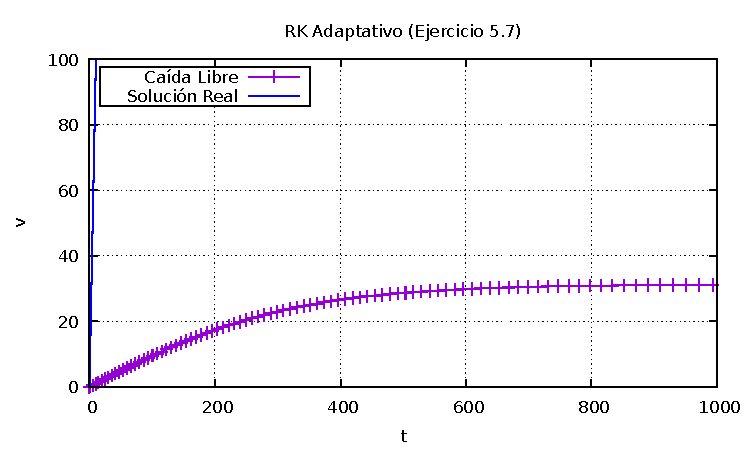
\includegraphics[scale=1]{../img/ej5-7.pdf}
	\caption{Gráfica para un objeto en caida libre con el método Runge Kutta adaptativo.}
	\label{ej5-7}
\end{figure}

\begin{lstlisting}
// Librerias
#include <iostream>
#include <cmath>
#include <iomanip>
#include <fstream>

// Librerias externas
#include "rkqs.hpp"
#include "odeint.hpp"

using namespace std;

void caidaLibreFriccion( double t, double *y, double *dydt );

int main(){
  int nvar, nok, nbad;
  double t1, t2, eps, h, hmin, *ystart;


  /* memory space for variables */
  // numero de ecuaciones
  nvar = 2;

  // valor inicial de cada variable
  ystart = new double[nvar];

  /* other variables initialization */
  // tolerancia (error)
  eps  = 1e-10;
  h    = 1;
  hmin = 1e-5;
  nok  = 0;
  nbad = 0;



  /* initial condition */
  ystart[0]  = 1.0;
  ystart[1]  = 0.0;

  // tiempo inicial
  t1 =  0.0;

  // tiempo final
  t2 =  2000.0;


  odeint(ystart, nvar, t1, t2, eps, h, hmin, &nok, &nbad, &caidaLibreFriccion, &rkqs);

  cout << "nok = " << nok <<"\t nbad = " << nbad << endl;

  return 0;
} // END main


void caidaLibreFriccion( double t, double *y, double *dydt ){
  const double g = 9.8;
  const double m = 0.01;
  const double k = .0001;


  dydt[0] = y[1];
  dydt[1] = g - (k/m)*y[1]*y[1];
} // END oneD_ProjectileMotion
\end{lstlisting}




\section*{Problema 3}
Se resuelve el oscilador de Ven der Pol
	$$ \ddot{x} = -x-\varepsilon (x^2 - 1) \dot{x}. $$
Se utiliza el método de Runge Kutta adaptativo. Tomando un $\varepsilon = 0$ no da una solución; sin embargo, si se utiliza un $h = 10^{-5}$, se tiene

\begin{figure}[H]
	\centering
	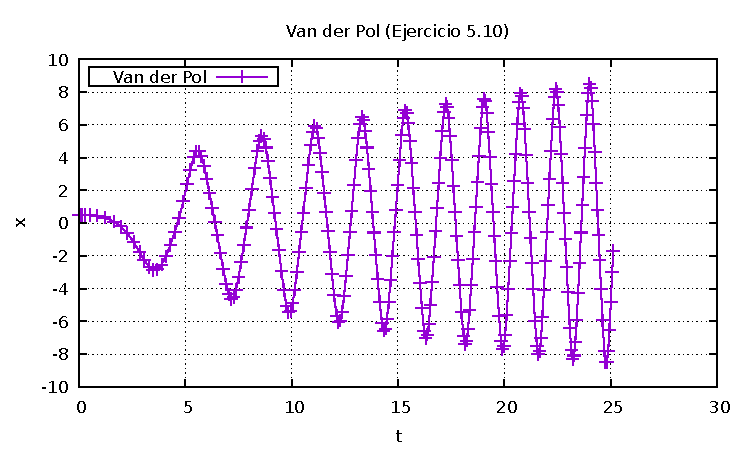
\includegraphics[scale=1]{../img/ej5-10.pdf}
	\caption{Solución para $x$ del oscilador Van der Pol.}
	\label{ej5-10}
\end{figure}

\begin{lstlisting}
// Librerias
#include <iostream>
#include <cmath>
#include <iomanip>
#include <fstream>

#include "rkqs.hpp"
#include "odeint.hpp"

using namespace std;


void VanderPol(double t, double *y, double *dydt);




int main(){
  int nvar, nok, nbad;
  double t1, t2, eps, h, hmin, *ystart;


  /* memory space for variables */
  // numero de ecuaciones
  nvar = 3;

  // valor inicial de cada variable
  ystart = new double[nvar];

  /* other variables initialization */
  // tolerancia (error)
  eps  = 1e-5;
  h    = 0.001;
  hmin = 1e-5;
  nok  = 0;
  nbad = 0;



  /* initial condition */
  ystart[0] = 0.5;
  ystart[1] = 0.0;
  ystart[2] = 0.0;

  // tiempo inicial
  t1 =  0.0;

  // tiempo final
  t2 =  25.12;


  odeint(ystart, nvar, t1, t2, eps, h, hmin, &nok, &nbad, &VanderPol, &rkqs);

  cout << "nok = " << nok <<"\t nbad = " << nbad << endl;

  return 0;
} // END main







void VanderPol(double t, double *y, double *dydt){
  dydt[0] = y[1];
  dydt[1] = y[2];
  dydt[2] = -y[0] - y[1]*(y[0]*y[0]-1);
} // END VanderPol

\end{lstlisting}


\section*{Problema 4}
Teniendo el sistema del péndulo simple
	$$ \ddot{\theta} = -\frac{g}{l} \sin{\theta}, $$
el cual se divide en dos ecuaciones diferenciales
	$$ \left\{\begin{array}{c}
		\dot{\theta} = \omega \\
		\dot{\omega} = -\frac{g}{l} \sin{\theta}
	\end{array}\right. .$$
Se encuentra la solución al mismo para ambas variables dependientes $\theta$ y $\dot{\theta}$. Se graficaron las mismas contra el tiempo y se graficó su diagrama de fase para las siguientes energías $E = 0.25$, $E =  0.5$, $E = 0.75$, $E = 1$, $E = 1.25$ y $E = 1.5$.

\begin{figure}[H]
	\centering
	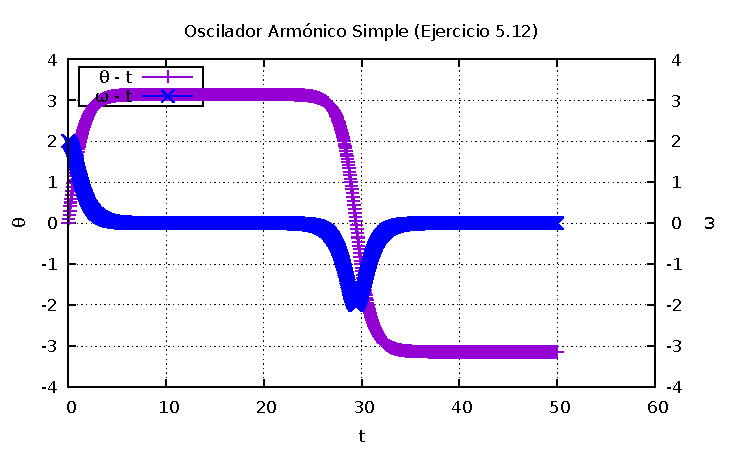
\includegraphics[scale=1]{../img/ej5-12-1.pdf}
	\caption{Gráfica de la posición angular y la velocidad angular.}
	\label{ej5-12-1}
\end{figure}

\begin{figure}[H]
	\centering
	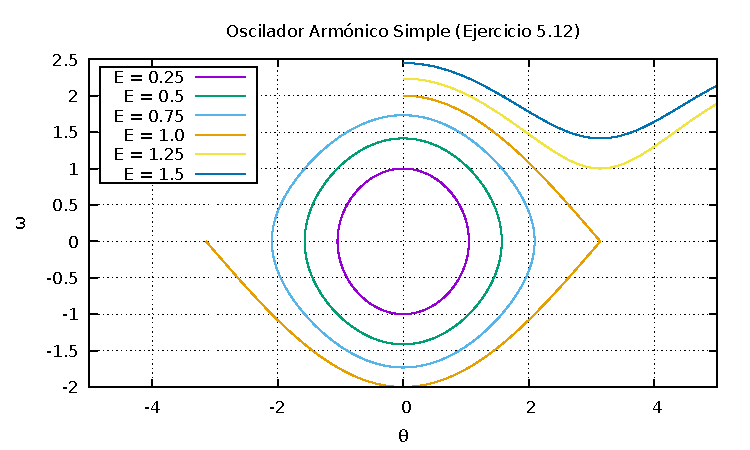
\includegraphics[scale=1]{../img/ej5-12-3.pdf}
	\caption{Gráfica de los diagramas de fase para las energías mostradas. Es claro que para la energía de $E = 1$, la trayectoria ya no es cerrada, esto implica que el péndulo no se comporta de la mejor forma y que la energía no se conserva, además de que salimos del rango en el que la aproximación de ángulos pequeños no es válida.}
	\label{ej5-12-1}
\end{figure}

\begin{lstlisting}
// Librerias
#include <iostream>
#include <fstream>
#include <cmath>
#include <iomanip>

using namespace std;


void RK4(const double *y,
		     const int n_ec,
		     const double t,
		     const double h,
		     double *y_new,
		     void (*derivada)(const double *, const double, double *));
void simple_oscilator(const double *y, const double t, double *dydt);




int main(){
  const double t0 = 0.0;
  const double y0 = 0.0;
  const double y1 = sqrt(6);
  const double h = 0.005;
  const int N = 10000;
  const int out_frec = 10;
  const int n_ec = 2;

  double t = t0;

  // espacio reservado
  double *y = new double[n_ec];
  double *y_nueva = new double[n_ec];

  void (*derivada)(const double *, const double, double *);
  derivada = simple_oscilator;

  for(int i = 0; i < n_ec; i++) y_nueva[i] = 0.0;

  y[0] = y0;
  y[1] = y1;

  cout << t << "\t" << y[0] << "\t" << y[1] << endl;

  for(int i = 0; i <= N; i++){
    RK4(y, n_ec, t, h, y_nueva, derivada);

    y = y_nueva;
    t += h;

    if (i % out_frec == 0){
      cout << t << "\t" << y[0] << "\t" << y[1] << endl;
    } // END IF
  } // END for

  return 0;
} // END main






void RK4(const double *y,
		     const int n_ec,
		     const double t,
		     const double h,
		     double *y_new,
		     void (*derivada)(const double *, const double, double *)){
  double *k0 = new double[ n_ec ];
  double *k1 = new double[ n_ec ];
  double *k2 = new double[ n_ec ];
  double *k3 = new double[ n_ec ];
  double *z  = new double[ n_ec ];

  (*derivada)( y, t, k0 );

  for( int i=0; i<n_ec; i++ )
    z[i] = y[i] + 0.5*k0[i]*h;

  (*derivada)( z, t+0.5*h, k1 );

  for( int i=0; i<n_ec; i++ )
    z[i] = y[i] + 0.5*k1[i]*h;

  (*derivada)( z, t+0.5*h, k2 );

  for( int i=0; i<n_ec; i++ )
    z[i] = y[i] + k2[i]*h;

  (*derivada)( z, t+h, k3 );

  for( int i=0; i<n_ec; i++ )
   y_new[i] = y[i] + h/6.0 * ( k0[i] + 2*k1[i] + 2*k2[i] + k3[i] );

  delete[] k0;
  delete[] k1;
  delete[] k2;
  delete[] k3;
  delete[] z;
} // END RK4


void simple_oscilator(const double *y, const double t, double *dydt){
  const double l = 1;
  const double g = 1;

  dydt[0] = y[1];
  dydt[1] = -(g/l)*sin(y[0]);
} // END simple_oscilator
\end{lstlisting}




\section*{Problema 5}
Para generar el video de la animación se utilizó \textit{gnuplot} para crear la todos los frames y se utilizó la librería \textbf{ffmpeg} para fusionar todos los frames en un archivo \textit{.mp4}, el resultado esta adjunto a este archivo en el espacio asignado en classroom.

\begin{lstlisting}
# En el directorio 'frames' donde estan las imagenes, ejecutar el siguiente
# comando, esto generara la animacion en un archivo .mp4
# ffmpeg -framerate 30 -pattern_type glob -i '*.png' -c:v libx264 -pix_fmt yuv420p out.mp4

# PROGRAM
set term pngcairo size 800,600 enhanced font "Verdana,12"


set xrange [-1:1]
set yrange [-1:1]
set xlabel 'x (m)'
set ylabel 'y (m)'


set size ratio -1

# longitud del pendulo
lon=1.0;

do for [i=0:1000] {
    set output sprintf( "frames/frame-%04d.png", i )
    set title sprintf( "tiempo = %f", i*0.02 )

    plot 'data2' every ::i::i u (x1=lon*sin($2)):(y1=-lon*cos($2)) w p lc 5 lw 5 t '', \
	 '' every ::i::i u (0.0):(0.0):(x1):(y1) w vectors nohead t ''

    print i
}
\end{lstlisting}




















%%%%%%%